\taughtsession{Lecture}{Relations}{2024-01-30}{17:00}{Janka}{}

\section{Ordered Pairs}
An ordered pair of elements is a group of two elements which are in a specific order. They are written as $(a, b)$ and the order matters - this means $(a, b)$ is distinct from the pair $(b, a)$. Note that ordered pairs use the brackets $()$ while sets use curly braces $\{\}$

\section{Cartesian Product}
The Cartesian Product of two sets is the set of \textbf{all} ordered pairs where the first element is taken from set 1 and the second element from set 2. The formal definition is as follows:
\[A \times B = \{(a, b) | a \in A \mathrm{\ and\ } b \in B\}\]
For example - if $X = \{1, 2, 3\}$ and $Y = \{a, b\}$, then
\[X \times Y = \{(1, a), (1, b), (2, a), (2, b), (3, a), (3, b)\}\]

\section{Relations}
A relation is the set of subsets from a cartesian product. For example, if we take $A = \{a, b, c, d, e\}$ and $B = {1, 2, 3}$ then:
\begin{align*}
    R_1 &= \{(a, 1), (b, 1), (c, 2), (c, 3)\}\\
    R_2 &= \{(a,3), (a,1),(c,2),(c,1),(b,2)\}
\end{align*}
$R_1$ and $R_2$ are both examples of Binary relations from A to B. 

\subsection{Describing Relations}
To describe a relation, we could list all of its elements, however this can be very long and obtuse so it's better \& more common practice to use ``the characteristics of their elements''. 

\subsection{Relations On A Set}
A relation \textit{on a set} is where both sets are equal. For example $A = B$ then a relation on $A$ is a relation from $A$ to $A$, hence a subset of $A \times A$. \\

For example, let $R$ be the relation on $A = \{1, 2, 3, 4\}$ as defined by:
\[(x, y) \in R \mathrm{\ if\ and\ only\ if\ } x \mathrm{\ divides\ } y\mathrm{,\ for\ all\ } x, y \in A \]
Then we can conclude that $R$ is:
\[R = \{(1,1), (1,2), (1,3), (1,4), (2,2), (2,4), (3,3), (4,4)\}\]

\section{A Digraph}
We can use a \textit{digraph} to picture a relation on a set. An example is shown below:
\begin{figure}[H]
    \centering
    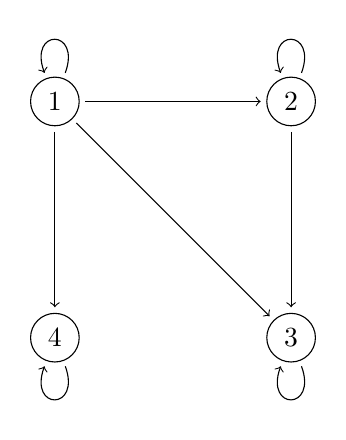
\begin{tikzpicture}[node distance=3cm]

    \node [circle, draw] (A) {1};
    \node [circle, draw] (B) [right of=A] {2};
    \node [circle, draw] (C) [below of=B] {3};
    \node [circle, draw] (D) [left of=C] {4};

    \draw[->, shorten >= 2pt, shorten <= 2pt] (A) -- (B);
    \draw[->, shorten >= 2pt, shorten <= 2pt] (B) -- (C);
    \draw[->, shorten >= 2pt, shorten <= 2pt] (A) -- (C);
    \draw[->, shorten >= 2pt, shorten <= 2pt] (A) -- (D);

    \draw[->, shorten >= 2pt, shorten <= 2pt] (A) edge [in=110, out=70,looseness=8] (A);
    \draw[->, shorten >= 2pt, shorten <= 2pt] (B) edge [in=110, out=70,looseness=8] (B);
    \draw[->, shorten >= 2pt, shorten <= 2pt] (D) edge [in=-110, out=-70,looseness=8] (D);
    \draw[->, shorten >= 2pt, shorten <= 2pt] (C) edge [in=-110, out=-70,looseness=8] (C);
    
    \end{tikzpicture}
\end{figure}

The dots (vertices) represents the elements of $A = \{1,2,3,4\}$. If the element $(x, y)$ is in the relation, an arrow (directed edge) is drawn from $x$ to $y$. 
\[R = \{(1,1), (1,2), (1,3), (1,4), (2,2), (2,4), (3,3), (4,4)\}\]

\subsection{Reflexivity}
A relation is reflexive where both elements in the ordered pair are the same element, for example $(1,1)$. In reference to the set $A = \{1, 2, 3, 4\}$, the relation:
\[R = {(1,1), (1,2), (1,3), (1,4), (2,2), (2,4), (3,3), (4,4)}\]
On the following digraph, the red arrows are the ones which display the reflexivity.
\begin{figure}[H]
    \centering
    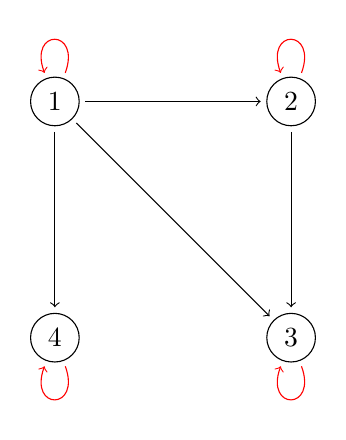
\begin{tikzpicture}[node distance=3cm]

    \node [circle, draw] (A) {1};
    \node [circle, draw] (B) [right of=A] {2};
    \node [circle, draw] (C) [below of=B] {3};
    \node [circle, draw] (D) [left of=C] {4};

    \draw[->, shorten >= 2pt, shorten <= 2pt] (A) -- (B);
    \draw[->, shorten >= 2pt, shorten <= 2pt] (B) -- (C);
    \draw[->, shorten >= 2pt, shorten <= 2pt] (A) -- (C);
    \draw[->, shorten >= 2pt, shorten <= 2pt] (A) -- (D);

    \draw[draw = red, ->, shorten >= 2pt, shorten <= 2pt] (A) edge [in=110, out=70,looseness=8] (A);
    \draw[draw = red,->, shorten >= 2pt, shorten <= 2pt] (B) edge [in=110, out=70,looseness=8] (B);
    \draw[draw = red,->, shorten >= 2pt, shorten <= 2pt] (D) edge [in=-110, out=-70,looseness=8] (D);
    \draw[draw = red,->, shorten >= 2pt, shorten <= 2pt] (C) edge [in=-110, out=-70,looseness=8] (C);
    
    \end{tikzpicture}
\end{figure}

\subsection{Symmetry}
A relation is symmetrical where $(x, y) \in R$ and $(y, x) \in R$. If the condition is not true, then we do not have symmetry.
\begin{figure}[H]
    \centering
    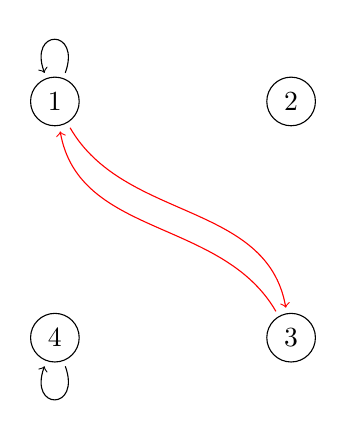
\begin{tikzpicture}[node distance=3cm]

    \node [circle, draw] (A) {1};
    \node [circle, draw] (B) [right of=A] {2};
    \node [circle, draw] (C) [below of=B] {3};
    \node [circle, draw] (D) [left of=C] {4};


    \draw[->, shorten >= 2pt, shorten <= 2pt] (A) edge [in=110, out=70,looseness=8] (A);
    \draw[->, shorten >= 2pt, shorten <= 2pt] (D) edge [in=-110, out=-70,looseness=8] (D);

    \draw[draw = red,->, shorten >= 2pt, shorten <= 2pt] (A) edge [in=100, out=-60] (C);
    \draw[draw = red,->, shorten >= 2pt, shorten <= 2pt] (C) edge [in=-80, out=120] (A);

    
    \end{tikzpicture}
\end{figure}

\subsection{Transitivity}
For a binary relation, $R$ on set $A$; $R$ is transitive if and only if for all $x, y, z \in A$ if $(x, y) \in R$ and $(y, z) \in R$ and $(x, z) \in R$.

\begin{figure}[H]
    \centering
    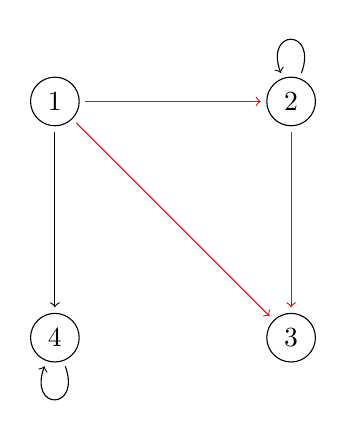
\begin{tikzpicture}[node distance=3cm]

    \node [circle, draw] (A) {1};
    \node [circle, draw] (B) [right of=A] {2};
    \node [circle, draw] (C) [below of=B] {3};
    \node [circle, draw] (D) [left of=C] {4};

    \draw[draw = red,->, shorten >= 2pt, shorten <= 2pt] (A) -- (B);
    \draw[draw = red,->, shorten >= 2pt, shorten <= 2pt] (B) -- (C);
    \draw[draw = red,->, shorten >= 2pt, shorten <= 2pt] (A) -- (C);
    \draw[->, shorten >= 2pt, shorten <= 2pt] (A) -- (D);

    \draw[->, shorten >= 2pt, shorten <= 2pt] (B) edge [in=110, out=70,looseness=8] (B);
    \draw[->, shorten >= 2pt, shorten <= 2pt] (D) edge [in=-110, out=-70,looseness=8] (D);
    
    \end{tikzpicture}
\end{figure}

\subsection{Equivalence}
Where a relation is reflexive, symmetric and transitive - it is classed as an equivalence. 

\subsubsection{Equivalence Class}
